% This is the Reed College LaTeX thesis template. Most of the work
% for the document class was done by Sam Noble (SN), as well as this
% template. Later comments etc. by Ben Salzberg (BTS). Additional
% restructuring and APA support by Jess Youngberg (JY).
% Your comments and suggestions are more than welcome; please email
% them to cus@reed.edu
%
% See https://www.reed.edu/cis/help/LaTeX/index.html for help. There are a
% great bunch of help pages there, with notes on
% getting started, bibtex, etc. Go there and read it if you're not
% already familiar with LaTeX.
%
% Any line that starts with a percent symbol is a comment.
% They won't show up in the document, and are useful for notes
% to yourself and explaining commands.
% Commenting also removes a line from the document;
% very handy for troubleshooting problems. -BTS

% As far as I know, this follows the requirements laid out in
% the 2002-2003 Senior Handbook. Ask a librarian to check the
% document before binding. -SN

%%
%% Preamble
%%
% \documentclass{<something>} must begin each LaTeX document
\documentclass[12pt,oneside,a4paper]{reedthesis}
% Packages are extensions to the basic LaTeX functions. Whatever you
% want to typeset, there is probably a package out there for it.
% Chemistry (chemtex), screenplays, you name it.
% Check out CTAN to see: https://www.ctan.org/
%%
\usepackage{amsmath}
\usepackage{graphicx,latexsym}
\usepackage{amssymb,amsthm}
\usepackage{longtable,booktabs,setspace}
\usepackage[hyphens]{url}
% Added by CII
\usepackage{hyperref}
\usepackage{lmodern}
\usepackage{float}
\floatplacement{figure}{H}
% End of CII addition
\usepackage{rotating}

% Next line commented out by CII
%%% \usepackage{natbib}
% Comment out the natbib line above and uncomment the following two lines to use the new
% biblatex-chicago style, for Chicago A. Also make some changes at the end where the
% bibliography is included.
%\usepackage{biblatex-chicago}
%\bibliography{thesis}

% Added by CII (Thanks, Hadley!)
% Use ref for internal links
\renewcommand{\hyperref}[2][???]{\autoref{#1}}
\def\chapterautorefname{Chapter}
\def\sectionautorefname{Section}
\def\subsectionautorefname{Subsection}
% End of CII addition

% Added by CII
\usepackage{caption}
\captionsetup{width=5in}
% End of CII addition

% \usepackage{times} % other fonts are available like times, bookman, charter, palatino

% Syntax highlighting #22
$if(highlighting-macros)$
  $highlighting-macros$
$endif$

% To pass between YAML and LaTeX the dollar signs are added by CII
\title{$title$}
\author{$author$}
% The month and year that you submit your FINAL draft TO THE LIBRARY (May or December)
\date{$date$}
\division{$division$}
\advisor{$advisor$}
\institution{$institution$}
\degree{$degree$}
%If you have two advisors for some reason, you can use the following
% Uncommented out by CII
$if(altadvisor)$
\altadvisor{$altadvisor$}
$endif$
% End of CII addition

% added by sç
\titleup{$titleup$}
\titletr{$titletr$}
\authorup{$authorup$}
\institutionup{$institutionup$}
\membera{$membera$}
\memberb{$memberb$}
\externala{$externala$}
\externalb{$externalb$}
\month{$month$}
\abstract{$abstract$}
\abstracttr{$abstracttr$}

%%% Remember to use the correct department!
\department{$department$}
% if you're writing a thesis in an interdisciplinary major,
% uncomment the line below and change the text as appropriate.
% check the Senior Handbook if unsure.
%\thedivisionof{The Established Interdisciplinary Committee for}
% if you want the approval page to say "Approved for the Committee",
% uncomment the next line
%\approvedforthe{Committee}

%sç
\usepackage[style=apa6]{biblatex}
\addbibresource{$bibliography$}

% Added by CII
%%% Copied from knitr
%% maxwidth is the original width if it's less than linewidth
%% otherwise use linewidth (to make sure the graphics do not exceed the margin)
\makeatletter
\def\maxwidth{ %
  \ifdim\Gin@nat@width>\linewidth
    \linewidth
  \else
    \Gin@nat@width
  \fi
}
\makeatother

%Added by @MyKo101, code provided by @GerbrichFerdinands
%$if(csl-refs)$
%\newlength{\cslhangindent}
%\setlength{\cslhangindent}{1.5em}
%\newenvironment{CSLReferences}%
%  {$if(csl-hanging-indent)$\setlength{\parindent}{0pt}%
%  \everypar{\setlength{\hangindent}{\cslhangindent}}\ignorespaces$endif$}%
%  {\par}
%$endif$

% for biblio entries, from the pandoc's template
\iftrue
\newlength{\cslhangindent}
\setlength{\cslhangindent}{1.5em}
\newlength{\cslentryspacingunit} % times entry-spacing
\setlength{\cslentryspacingunit}{1em}
\newenvironment{CSLReferences}[2] % #1 hanging-ident, #2 entry spacing
 {% don't indent paragraphs
  \setlength{\parindent}{0pt}
  % turn on hanging indent if param 1 is 1
  \ifodd #1
  \let\oldpar\par
  \def\par{\hangindent=\cslhangindent\oldpar}
  \fi
  \par
  % set entry spacing
  %\setlength{\parskip}{#2\cslentryspacingunit}
 }%
 
\newenvironment{cslreferences}[2] % #1 hanging-ident, #2 entry spacing
 {% don't indent paragraphs
  \setlength{\parindent}{0pt}
  % turn on hanging indent if param 1 is 1
  \ifodd #1
  \let\oldpar\par
  \def\par{\hangindent=\cslhangindent\oldpar}
  \fi
  % set entry spacing
  \setlength{\parskip}{#2\cslentryspacingunit}
 }%
\fi


\renewcommand{\contentsname}{Table of Contents}
% End of CII addition

\setlength{\parskip}{0pt}

% Added by CII
$if(space_between_paragraphs)$
  %\setlength{\parskip}{\baselineskip}
  \usepackage[parfill]{parskip}
$endif$

\providecommand{\tightlist}{%
  \setlength{\itemsep}{0pt}\setlength{\parskip}{0pt}}

\Acknowledgements{
$acknowledgements$
}

\Dedication{
$dedication$
}

\Preface{
$preface$
}

\Abstract{
$abstract$
}

$for(header-includes)$
	$header-includes$
$endfor$
% End of CII addition
%%
%% End Preamble
%%
%
\begin{document}

%\pagestyle{empty}
%$if(titleup)$
%  \makecover
%$endif$

\pagestyle{empty}
\begin{coverpage}
  \centering
  \vspace*{\fill}
  $titleup$\\
  \vspace{7.5cm}
  $authorup$\\
  \vspace{7.5cm}
  $institutionup$\\
  $date$
  \vspace*{\fill}
\end{coverpage}

%\frontmatter % this stuff will be roman-numbered

% Everything below added by CII
%$if(title)$
%  \maketitle
%$endif$

\newpage
\begin{titlepag2}
  \centering
  \vspace*{\fill}
  $titleup$\\
  \vspace{2.6cm}
  Thesis submitted to the\\
  $division$\\
  in partial fulfillment of the requirements for the degree of\\
  \vspace{2cm}
  $degree$\\
  in\\
  $department$\\
  \vspace{1.9cm}
  by\\
  $author$\\
  \vspace{3.8cm}
  $institution$\\
  $date$
  \vspace*{\fill}
\end{titlepag2}

\setcounter{page}{1}
\renewcommand{\thepage}{\roman{page}}% Roman numerals for page counter

%\makeapproval
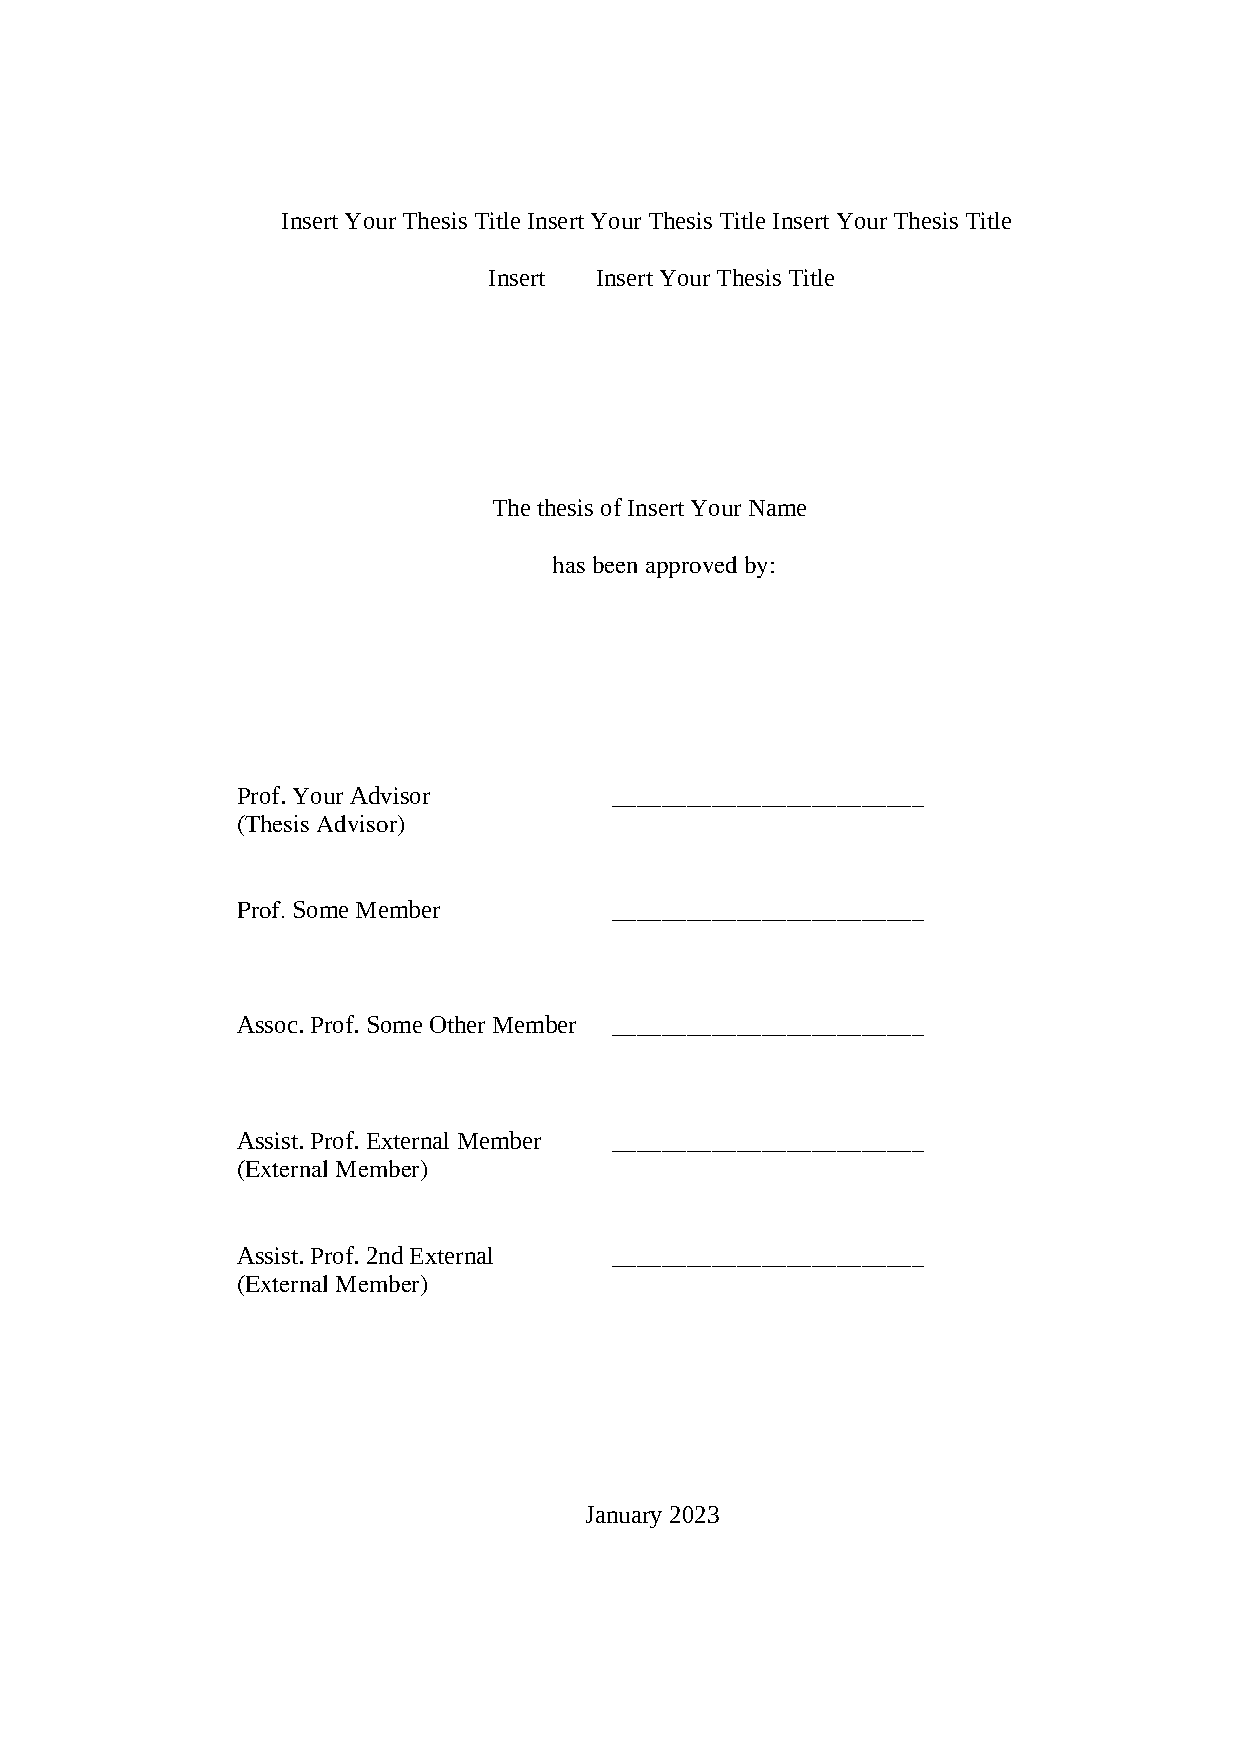
\includepdf[pages=-]{approval_page.pdf}

\includepdf[pages=2]{f1_declaration_of_originality.pdf}

\pagestyle{plain} % this removes page numbers from the frontmatter

\newpage
\makeabstract

\newpage
\makeabstracttr

\newpage
\begin{cve}
{\setlength{\parindent}{0pt}
$cv$
}
\end{cve}

\newpage
$acknow$

\newpage
\begin{dedice}
{\setlength{\parskip}{18pt}
\vspace*{\fill}
\raggedleft{\itshape $dedication$}
\par
\vspace*{\fill}
}
\end{dedice}

$if(acknowledgements)$
  \begin{acknowledgements}
    $acknowledgements$
  \end{acknowledgements}
$endif$

$if(preface)$
  \begin{preface}
    $preface$
  \end{preface}
$endif$

$if(toc)$
  \hypersetup{linkcolor=$if(toccolor)$$toccolor$$else$black$endif$}
  \setcounter{secnumdepth}{$num-depth$}
  \setcounter{tocdepth}{$toc-depth$}
  \tableofcontents
$endif$

$if(lot)$
  \listoftables
$endif$

$if(lof)$
  \listoffigures
$endif$

\newpage
\begin{abbre}
{\setlength{\parindent}{0pt}
$abbr$
}
\end{abbre}
\newpage
\setcounter{table}{0}

\setcounter{page}{1}
\mainmatter % here the regular arabic numbering starts
\pagestyle{plain} % turns page numbering back on
\renewcommand{\thepage}{\arabic{page}}% Roman numerals for page counter

$body$

\begingroup
\begin{singlespace}
\printbibliography[title=REFERENCES, heading=bibintoc]
\end{singlespace}
\endgroup

\end{document}

